\documentclass{standalone}
\usepackage{tikz}
\usetikzlibrary{calc}
\usetikzlibrary{intersections}

\begin{document}

\centering

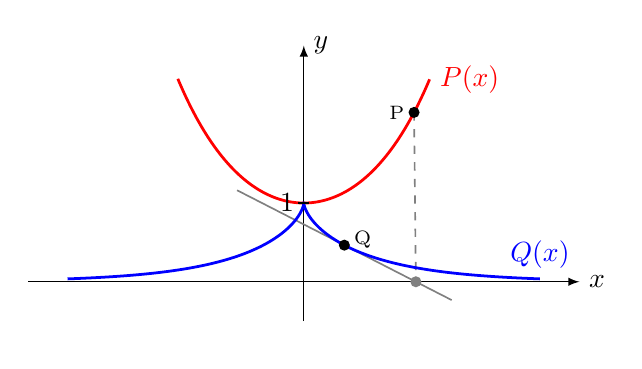
\begin{tikzpicture}
    % draw axes
    \coordinate (O) at (0,0);
    \draw[-latex] (0,-0.5) -- (0,3) node[anchor=west] {$y$};
    \draw[-latex] (-3.5,0) -- (3.5,0) node[anchor=west] {$x$};

    % define functions
    \def\a{1} % constant
    % CATENARY
    \pgfmathdeclarefunction{catenaryY}{1}{%
    \pgfmathparse{\a*cosh(#1/\a)}%
    }
    % TRACTRIX
    \pgfmathdeclarefunction{tractrixX}{1}{%
    \pgfmathparse{#1 - \a*tanh(#1/\a)}%
    }
    \pgfmathdeclarefunction{tractrixY}{1}{%
    \pgfmathparse{\a/cosh(#1/\a)}%
    }

     % tractrix couple example
    % INPUT: set x-coordinate
    \pgfmathsetmacro{\XExample}{1.4}

    % corresponding coordinate on the catenary
    \pgfmathsetmacro{\PXExample}{\XExample}
    \pgfmathsetmacro{\PYExample}{catenaryY{\XExample}}
    \coordinate (PExample) at (\PXExample, \PYExample);
     % corresponding coordinate on the tractrix
    \pgfmathsetmacro{\QXExample}{tractrixX{\XExample}}
    \pgfmathsetmacro{\QYExample}{tractrixY{\XExample}}
    \coordinate (QExample) at (\QXExample, \QYExample);

    % draw tangent (via epsilon increase)
    % define point at an epsilon increase
    \pgfmathsetmacro{\Eps}{0.05}
    \pgfmathsetmacro{\Extrapolate}{3 / \Eps}
    \pgfmathsetmacro{\XTangent}{\XExample+\Eps}
    % corresponding coordinate
    \pgfmathsetmacro{\QXTangent}{tractrixX{\XTangent}}
    \pgfmathsetmacro{\QYTangent}{tractrixY{\XTangent}}
    \coordinate (QTangent) at (\QXTangent, \QYTangent);

    % determine the intersection point between tangent and x-axis
    % extrapolate from the two points to get the tangent
    \path[name path=TangentTractrix] (QExample) -- ($(QExample)!\Extrapolate!(QTangent)$);
    % define path for x-axis
    \path[name path=XAxis] (-3.5, 0) -- (3.5, 0);
    % intersection tangent and x-axis
    \path[name intersections={of=TangentTractrix and XAxis, by=Intersection}];

    % draw the tangent line
    \draw[gray, semithick] ($(Intersection)!2.5!(QExample)$) -- ($(QExample)!1.5!(Intersection)$);
    % draw intersection point
    \fill[gray] (Intersection) circle [radius=2pt];

    % draw the X-projection
    \draw[dashed, semithick, gray] (PExample) -- (Intersection);


    % DRAW THE CURVES: CATNEARY AND TRACTRIX
    
    \draw[red,domain=-1.6:1.6,samples=200, line width=1, smooth] plot ({\x},catenaryY{\x}) node[right] {$P(x)$};

    \draw[blue,domain=-4:4,samples=200, line width=1, smooth] plot (tractrixX{\x},tractrixY{\x}) node[above] {$Q(x)$};

    % draw labels
    \node[anchor=east] at (0,1) {$1$};
    \draw (-2pt,1) -- (2pt,1);

     % draw both coordinates
    \fill (PExample) circle[radius=2.0pt] node[above, left, font=\scriptsize] {P};
    \fill (QExample) circle[radius=2.0pt] node[above, right, yshift=2pt, font=\scriptsize] {Q};

   

    
\end{tikzpicture}

\end{document}